\documentclass[1p]{elsarticle_modified}
%\bibliographystyle{elsarticle-num}

%\usepackage[colorlinks]{hyperref}
%\usepackage{abbrmath_seonhwa} %\Abb, \Ascr, \Acal ,\Abf, \Afrak
\usepackage{amsfonts}
\usepackage{amssymb}
\usepackage{amsmath}
\usepackage{amsthm}
\usepackage{scalefnt}
\usepackage{amsbsy}
\usepackage{kotex}
\usepackage{caption}
\usepackage{subfig}
\usepackage{color}
\usepackage{graphicx}
\usepackage{xcolor} %% white, black, red, green, blue, cyan, magenta, yellow
\usepackage{float}
\usepackage{setspace}
\usepackage{hyperref}

\usepackage{tikz}
\usetikzlibrary{arrows}

\usepackage{multirow}
\usepackage{array} % fixed length table
\usepackage{hhline}

%%%%%%%%%%%%%%%%%%%%%
\makeatletter
\renewcommand*\env@matrix[1][\arraystretch]{%
	\edef\arraystretch{#1}%
	\hskip -\arraycolsep
	\let\@ifnextchar\new@ifnextchar
	\array{*\c@MaxMatrixCols c}}
\makeatother %https://tex.stackexchange.com/questions/14071/how-can-i-increase-the-line-spacing-in-a-matrix
%%%%%%%%%%%%%%%

\usepackage[normalem]{ulem}

\newcommand{\msout}[1]{\ifmmode\text{\sout{\ensuremath{#1}}}\else\sout{#1}\fi}
%SOURCE: \msout is \stkout macro in https://tex.stackexchange.com/questions/20609/strikeout-in-math-mode

\newcommand{\cancel}[1]{
	\ifmmode
	{\color{red}\msout{#1}}
	\else
	{\color{red}\sout{#1}}
	\fi
}

\newcommand{\add}[1]{
	{\color{blue}\uwave{#1}}
}

\newcommand{\replace}[2]{
	\ifmmode
	{\color{red}\msout{#1}}{\color{blue}\uwave{#2}}
	\else
	{\color{red}\sout{#1}}{\color{blue}\uwave{#2}}
	\fi
}

\newcommand{\Sol}{\mathcal{S}} %segment
\newcommand{\D}{D} %diagram
\newcommand{\A}{\mathcal{A}} %arc


%%%%%%%%%%%%%%%%%%%%%%%%%%%%%5 test

\def\sl{\operatorname{\textup{SL}}(2,\Cbb)}
\def\psl{\operatorname{\textup{PSL}}(2,\Cbb)}
\def\quan{\mkern 1mu \triangleright \mkern 1mu}

\theoremstyle{definition}
\newtheorem{thm}{Theorem}[section]
\newtheorem{prop}[thm]{Proposition}
\newtheorem{lem}[thm]{Lemma}
\newtheorem{ques}[thm]{Question}
\newtheorem{cor}[thm]{Corollary}
\newtheorem{defn}[thm]{Definition}
\newtheorem{exam}[thm]{Example}
\newtheorem{rmk}[thm]{Remark}
\newtheorem{alg}[thm]{Algorithm}

\newcommand{\I}{\sqrt{-1}}
\begin{document}

%\begin{frontmatter}
%
%\title{Boundary parabolic representations of knots up to 8 crossings}
%
%%% Group authors per affiliation:
%\author{Yunhi Cho} 
%\address{Department of Mathematics, University of Seoul, Seoul, Korea}
%\ead{yhcho@uos.ac.kr}
%
%
%\author{Seonhwa Kim} %\fnref{s_kim}}
%\address{Center for Geometry and Physics, Institute for Basic Science, Pohang, 37673, Korea}
%\ead{ryeona17@ibs.re.kr}
%
%\author{Hyuk Kim}
%\address{Department of Mathematical Sciences, Seoul National University, Seoul 08826, Korea}
%\ead{hyukkim@snu.ac.kr}
%
%\author{Seokbeom Yoon}
%\address{Department of Mathematical Sciences, Seoul National University, Seoul, 08826,  Korea}
%\ead{sbyoon15@snu.ac.kr}
%
%\begin{abstract}
%We find all boundary parabolic representation of knots up to 8 crossings.
%
%\end{abstract}
%\begin{keyword}
%    \MSC[2010] 57M25 
%\end{keyword}
%
%\end{frontmatter}

%\linenumbers
%\tableofcontents
%
\newcommand\colored[1]{\textcolor{white}{\rule[-0.35ex]{0.8em}{1.4ex}}\kern-0.8em\color{red} #1}%
%\newcommand\colored[1]{\textcolor{white}{ #1}\kern-2.17ex	\textcolor{white}{ #1}\kern-1.81ex	\textcolor{white}{ #1}\kern-2.15ex\color{red}#1	}

{\Large $\underline{12n_{0240}~(K12n_{0240})}$}

\setlength{\tabcolsep}{10pt}
\renewcommand{\arraystretch}{1.6}
\vspace{1cm}\begin{tabular}{m{100pt}>{\centering\arraybackslash}m{274pt}}
\multirow{5}{120pt}{
	\centering
	\includegraphics[width=112pt]{../../../GIT/diagram.site/Diagrams/png/2329_12n_0240.png}\\
\ \ \ A knot diagram\footnotemark}&
\allowdisplaybreaks
\textbf{Linearized knot diagam} \\
\cline{2-2}
 &
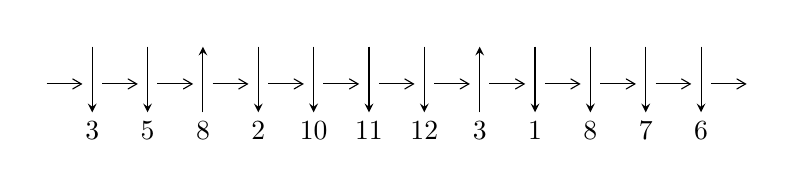
\begin{tikzpicture}[x=20pt, y=17pt]
	% nodes
	\node (C0) at (0, 0) {};
	\node (C1) at (1, 0) {};
	\node (C1U) at (1, +1) {};
	\node (C1D) at (1, -1) {3};

	\node (C2) at (2, 0) {};
	\node (C2U) at (2, +1) {};
	\node (C2D) at (2, -1) {5};

	\node (C3) at (3, 0) {};
	\node (C3U) at (3, +1) {};
	\node (C3D) at (3, -1) {8};

	\node (C4) at (4, 0) {};
	\node (C4U) at (4, +1) {};
	\node (C4D) at (4, -1) {2};

	\node (C5) at (5, 0) {};
	\node (C5U) at (5, +1) {};
	\node (C5D) at (5, -1) {10};

	\node (C6) at (6, 0) {};
	\node (C6U) at (6, +1) {};
	\node (C6D) at (6, -1) {11};

	\node (C7) at (7, 0) {};
	\node (C7U) at (7, +1) {};
	\node (C7D) at (7, -1) {12};

	\node (C8) at (8, 0) {};
	\node (C8U) at (8, +1) {};
	\node (C8D) at (8, -1) {3};

	\node (C9) at (9, 0) {};
	\node (C9U) at (9, +1) {};
	\node (C9D) at (9, -1) {1};

	\node (C10) at (10, 0) {};
	\node (C10U) at (10, +1) {};
	\node (C10D) at (10, -1) {8};

	\node (C11) at (11, 0) {};
	\node (C11U) at (11, +1) {};
	\node (C11D) at (11, -1) {7};

	\node (C12) at (12, 0) {};
	\node (C12U) at (12, +1) {};
	\node (C12D) at (12, -1) {6};
	\node (C13) at (13, 0) {};

	% arrows
	\draw[->,>={angle 60}]
	(C0) edge (C1) (C1) edge (C2) (C2) edge (C3) (C3) edge (C4) (C4) edge (C5) (C5) edge (C6) (C6) edge (C7) (C7) edge (C8) (C8) edge (C9) (C9) edge (C10) (C10) edge (C11) (C11) edge (C12) (C12) edge (C13) ;	\draw[->,>=stealth]
	(C1U) edge (C1D) (C2U) edge (C2D) (C3D) edge (C3U) (C4U) edge (C4D) (C5U) edge (C5D) (C6U) edge (C6D) (C7U) edge (C7D) (C8D) edge (C8U) (C9U) edge (C9D) (C10U) edge (C10D) (C11U) edge (C11D) (C12U) edge (C12D) ;
	\end{tikzpicture} \\
\hhline{~~} \\& 
\textbf{Solving Sequence} \\ \cline{2-2} 
 &
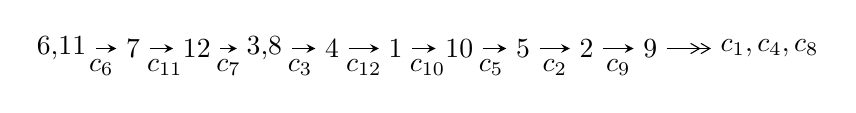
\begin{tikzpicture}[x=23pt, y=7pt]
	% node
	\node (A0) at (-1/8, 0) {6,11};
	\node (A1) at (1, 0) {7};
	\node (A2) at (2, 0) {12};
	\node (A3) at (49/16, 0) {3,8};
	\node (A4) at (33/8, 0) {4};
	\node (A5) at (41/8, 0) {1};
	\node (A6) at (49/8, 0) {10};
	\node (A7) at (57/8, 0) {5};
	\node (A8) at (65/8, 0) {2};
	\node (A9) at (73/8, 0) {9};
	\node (C1) at (1/2, -1) {$c_{6}$};
	\node (C2) at (3/2, -1) {$c_{11}$};
	\node (C3) at (5/2, -1) {$c_{7}$};
	\node (C4) at (29/8, -1) {$c_{3}$};
	\node (C5) at (37/8, -1) {$c_{12}$};
	\node (C6) at (45/8, -1) {$c_{10}$};
	\node (C7) at (53/8, -1) {$c_{5}$};
	\node (C8) at (61/8, -1) {$c_{2}$};
	\node (C9) at (69/8, -1) {$c_{9}$};
	\node (A10) at (11, 0) {$c_{1},c_{4},c_{8}$};

	% edge
	\draw[->,>=stealth]	
	(A0) edge (A1) (A1) edge (A2) (A2) edge (A3) (A3) edge (A4) (A4) edge (A5) (A5) edge (A6) (A6) edge (A7) (A7) edge (A8) (A8) edge (A9) ;
	\draw[->>,>={angle 60}]	
	(A9) edge (A10);
\end{tikzpicture} \\ 

\end{tabular} \\

\footnotetext{
The image of knot diagram is generated by the software ``\textbf{Draw programme}" developed by Andrew Bartholomew(\url{http://www.layer8.co.uk/maths/draw/index.htm\#Running-draw}), where we modified some parts for our purpose(\url{https://github.com/CATsTAILs/LinksPainter}).
}\phantom \\ \newline 
\centering \textbf{Ideals for irreducible components\footnotemark of $X_{\text{par}}$} 
 
\begin{align*}
I^u_{1}&=\langle 
- u^{45}+u^{44}+\cdots+b+2 u,\;-2 u^{45}+2 u^{44}+\cdots+a+8 u,\;u^{46}-2 u^{45}+\cdots+u+1\rangle \\
I^u_{2}&=\langle 
u^3+b- u+1,\;u^6-3 u^4+2 u^2+a+1,\;u^8+u^7-3 u^6-2 u^5+3 u^4+2 u-1\rangle \\
\\
\end{align*}
\raggedright * 2 irreducible components of $\dim_{\mathbb{C}}=0$, with total 54 representations.\\
\footnotetext{All coefficients of polynomials are rational numbers. But the coefficients are sometimes approximated in decimal forms when there is not enough margin.}
\newpage
\renewcommand{\arraystretch}{1}
\centering \section*{I. $I^u_{1}= \langle - u^{45}+u^{44}+\cdots+b+2 u,\;-2 u^{45}+2 u^{44}+\cdots+a+8 u,\;u^{46}-2 u^{45}+\cdots+u+1 \rangle$}
\flushleft \textbf{(i) Arc colorings}\\
\begin{tabular}{m{7pt} m{180pt} m{7pt} m{180pt} }
\flushright $a_{6}=$&$\begin{pmatrix}1\\0\end{pmatrix}$ \\
\flushright $a_{11}=$&$\begin{pmatrix}0\\u\end{pmatrix}$ \\
\flushright $a_{7}=$&$\begin{pmatrix}1\\u^2\end{pmatrix}$ \\
\flushright $a_{12}=$&$\begin{pmatrix}- u\\- u^3+u\end{pmatrix}$ \\
\flushright $a_{3}=$&$\begin{pmatrix}2 u^{45}-2 u^{44}+\cdots+10 u^2-8 u\\u^{45}- u^{44}+\cdots+5 u^2-2 u\end{pmatrix}$ \\
\flushright $a_{8}=$&$\begin{pmatrix}- u^2+1\\- u^4+2 u^2\end{pmatrix}$ \\
\flushright $a_{4}=$&$\begin{pmatrix}4 u^{45}-4 u^{44}+\cdots-10 u-1\\u^{45}- u^{44}+\cdots+4 u^2-3 u\end{pmatrix}$ \\
\flushright $a_{1}=$&$\begin{pmatrix}u^3-2 u\\- u^3+u\end{pmatrix}$ \\
\flushright $a_{10}=$&$\begin{pmatrix}u^5-2 u^3+u\\u^7-3 u^5+2 u^3+u\end{pmatrix}$ \\
\flushright $a_{5}=$&$\begin{pmatrix}- u^{12}+5 u^{10}-9 u^8+6 u^6- u^2+1\\- u^{14}+6 u^{12}-13 u^{10}+10 u^8+2 u^6-4 u^4- u^2\end{pmatrix}$ \\
\flushright $a_{2}=$&$\begin{pmatrix}u^{45}- u^{44}+\cdots-8 u+1\\u^{45}- u^{44}+\cdots+5 u^2- u\end{pmatrix}$ \\
\flushright $a_{9}=$&$\begin{pmatrix}u^{13}-6 u^{11}+13 u^9-10 u^7-2 u^5+4 u^3+u\\- u^{13}+5 u^{11}-9 u^9+6 u^7- u^3+u\end{pmatrix}$\\&\end{tabular}
\flushleft \textbf{(ii) Obstruction class $= -1$}\\~\\
\flushleft \textbf{(iii) Cusp Shapes $= -3 u^{45}+56 u^{43}+\cdots-5 u-1$}\\~\\
\newpage\renewcommand{\arraystretch}{1}
\flushleft \textbf{(iv) u-Polynomials at the component}\newline \\
\begin{tabular}{m{50pt}|m{274pt}}
Crossings & \hspace{64pt}u-Polynomials at each crossing \\
\hline $$\begin{aligned}c_{1}\end{aligned}$$&$\begin{aligned}
&u^{46}+11 u^{45}+\cdots+25 u+1
\end{aligned}$\\
\hline $$\begin{aligned}c_{2},c_{4}\end{aligned}$$&$\begin{aligned}
&u^{46}-9 u^{45}+\cdots-9 u+1
\end{aligned}$\\
\hline $$\begin{aligned}c_{3},c_{8}\end{aligned}$$&$\begin{aligned}
&u^{46}+u^{45}+\cdots+1152 u+256
\end{aligned}$\\
\hline $$\begin{aligned}c_{5}\end{aligned}$$&$\begin{aligned}
&u^{46}-2 u^{45}+\cdots+2660 u+1960
\end{aligned}$\\
\hline $$\begin{aligned}c_{6},c_{7},c_{11}\end{aligned}$$&$\begin{aligned}
&u^{46}+2 u^{45}+\cdots- u+1
\end{aligned}$\\
\hline $$\begin{aligned}c_{9}\end{aligned}$$&$\begin{aligned}
&u^{46}+2 u^{45}+\cdots+7 u+1
\end{aligned}$\\
\hline $$\begin{aligned}c_{10},c_{12}\end{aligned}$$&$\begin{aligned}
&u^{46}-6 u^{45}+\cdots-73 u+17
\end{aligned}$\\
\hline
\end{tabular}\\~\\
\newpage\renewcommand{\arraystretch}{1}
\flushleft \textbf{(v) Riley Polynomials at the component}\newline \\
\begin{tabular}{m{50pt}|m{274pt}}
Crossings & \hspace{64pt}Riley Polynomials at each crossing \\
\hline $$\begin{aligned}c_{1}\end{aligned}$$&$\begin{aligned}
&y^{46}+57 y^{45}+\cdots-21 y+1
\end{aligned}$\\
\hline $$\begin{aligned}c_{2},c_{4}\end{aligned}$$&$\begin{aligned}
&y^{46}-11 y^{45}+\cdots-25 y+1
\end{aligned}$\\
\hline $$\begin{aligned}c_{3},c_{8}\end{aligned}$$&$\begin{aligned}
&y^{46}-51 y^{45}+\cdots-1490944 y+65536
\end{aligned}$\\
\hline $$\begin{aligned}c_{5}\end{aligned}$$&$\begin{aligned}
&y^{46}+18 y^{45}+\cdots-21367920 y+3841600
\end{aligned}$\\
\hline $$\begin{aligned}c_{6},c_{7},c_{11}\end{aligned}$$&$\begin{aligned}
&y^{46}-38 y^{45}+\cdots-17 y+1
\end{aligned}$\\
\hline $$\begin{aligned}c_{9}\end{aligned}$$&$\begin{aligned}
&y^{46}+54 y^{45}+\cdots-17 y+1
\end{aligned}$\\
\hline $$\begin{aligned}c_{10},c_{12}\end{aligned}$$&$\begin{aligned}
&y^{46}+34 y^{45}+\cdots-5737 y+289
\end{aligned}$\\
\hline
\end{tabular}\\~\\
\newpage\flushleft \textbf{(vi) Complex Volumes and Cusp Shapes}
$$\begin{array}{c|c|c}  
\text{Solutions to }I^u_{1}& \I (\text{vol} + \sqrt{-1}CS) & \text{Cusp shape}\\
 \hline 
\begin{aligned}
u &= -0.088878 + 0.844041 I \\
a &= \phantom{-}3.37742 - 1.22551 I \\
b &= -2.98228 + 0.61868 I\end{aligned}
 & \phantom{-}11.39320 + 1.80249 I & -2.43037 - 0.91952 I \\ \hline\begin{aligned}
u &= -0.088878 - 0.844041 I \\
a &= \phantom{-}3.37742 + 1.22551 I \\
b &= -2.98228 - 0.61868 I\end{aligned}
 & \phantom{-}11.39320 - 1.80249 I & -2.43037 + 0.91952 I \\ \hline\begin{aligned}
u &= -0.116026 + 0.837306 I \\
a &= -3.46305 + 1.35399 I \\
b &= \phantom{-}3.14660 - 0.77902 I\end{aligned}
 & \phantom{-}10.46260 + 9.14915 I & -3.66280 - 5.53840 I \\ \hline\begin{aligned}
u &= -0.116026 - 0.837306 I \\
a &= -3.46305 - 1.35399 I \\
b &= \phantom{-}3.14660 + 0.77902 I\end{aligned}
 & \phantom{-}10.46260 - 9.14915 I & -3.66280 + 5.53840 I \\ \hline\begin{aligned}
u &= \phantom{-}1.141830 + 0.219995 I \\
a &= -0.660574 + 0.098342 I \\
b &= -0.127713 - 0.217138 I\end{aligned}
 & -1.38478 - 0.54129 I & -5.73844 + 0. I\phantom{ +0.000000I} \\ \hline\begin{aligned}
u &= \phantom{-}1.141830 - 0.219995 I \\
a &= -0.660574 - 0.098342 I \\
b &= -0.127713 + 0.217138 I\end{aligned}
 & -1.38478 + 0.54129 I & -5.73844 + 0. I\phantom{ +0.000000I} \\ \hline\begin{aligned}
u &= \phantom{-}0.058004 + 0.794656 I \\
a &= \phantom{-}1.48803 - 0.66681 I \\
b &= -1.176270 + 0.234722 I\end{aligned}
 & \phantom{-}3.97447 - 2.81253 I & -2.78364 + 4.01547 I \\ \hline\begin{aligned}
u &= \phantom{-}0.058004 - 0.794656 I \\
a &= \phantom{-}1.48803 + 0.66681 I \\
b &= -1.176270 - 0.234722 I\end{aligned}
 & \phantom{-}3.97447 + 2.81253 I & -2.78364 - 4.01547 I \\ \hline\begin{aligned}
u &= -1.139460 + 0.393221 I \\
a &= -1.60826 + 1.63861 I \\
b &= \phantom{-}2.48711 + 1.35446 I\end{aligned}
 & \phantom{-}7.33193 - 4.71190 I & -6.52326 + 0. I\phantom{ +0.000000I} \\ \hline\begin{aligned}
u &= -1.139460 - 0.393221 I \\
a &= -1.60826 - 1.63861 I \\
b &= \phantom{-}2.48711 - 1.35446 I\end{aligned}
 & \phantom{-}7.33193 + 4.71190 I & -6.52326 + 0. I\phantom{ +0.000000I}\\
 \hline 
 \end{array}$$\newpage$$\begin{array}{c|c|c}  
\text{Solutions to }I^u_{1}& \I (\text{vol} + \sqrt{-1}CS) & \text{Cusp shape}\\
 \hline 
\begin{aligned}
u &= -1.175260 + 0.396885 I \\
a &= \phantom{-}1.58950 - 1.52874 I \\
b &= -2.60724 - 1.21777 I\end{aligned}
 & \phantom{-}8.06092 + 2.65955 I & \phantom{-0.000000 } 0 \\ \hline\begin{aligned}
u &= -1.175260 - 0.396885 I \\
a &= \phantom{-}1.58950 + 1.52874 I \\
b &= -2.60724 + 1.21777 I\end{aligned}
 & \phantom{-}8.06092 - 2.65955 I & \phantom{-0.000000 } 0 \\ \hline\begin{aligned}
u &= -0.027447 + 0.752835 I \\
a &= -2.58406 - 0.48560 I \\
b &= \phantom{-}1.92495 + 0.96879 I\end{aligned}
 & \phantom{-}1.16885 + 1.15848 I & -5.01072 + 0.12391 I \\ \hline\begin{aligned}
u &= -0.027447 - 0.752835 I \\
a &= -2.58406 + 0.48560 I \\
b &= \phantom{-}1.92495 - 0.96879 I\end{aligned}
 & \phantom{-}1.16885 - 1.15848 I & -5.01072 - 0.12391 I \\ \hline\begin{aligned}
u &= \phantom{-}0.135112 + 0.737338 I \\
a &= -0.263549 - 0.833035 I \\
b &= \phantom{-}0.030415 + 0.576766 I\end{aligned}
 & \phantom{-}1.53760 - 3.03900 I & -1.98360 + 5.04098 I \\ \hline\begin{aligned}
u &= \phantom{-}0.135112 - 0.737338 I \\
a &= -0.263549 + 0.833035 I \\
b &= \phantom{-}0.030415 - 0.576766 I\end{aligned}
 & \phantom{-}1.53760 + 3.03900 I & -1.98360 - 5.04098 I \\ \hline\begin{aligned}
u &= \phantom{-}1.215480 + 0.337571 I \\
a &= \phantom{-}0.103389 + 1.085520 I \\
b &= -0.822594 + 0.083089 I\end{aligned}
 & \phantom{-}0.425497 - 1.277230 I & \phantom{-0.000000 } 0 \\ \hline\begin{aligned}
u &= \phantom{-}1.215480 - 0.337571 I \\
a &= \phantom{-}0.103389 - 1.085520 I \\
b &= -0.822594 - 0.083089 I\end{aligned}
 & \phantom{-}0.425497 + 1.277230 I & \phantom{-0.000000 } 0 \\ \hline\begin{aligned}
u &= -1.259210 + 0.309211 I \\
a &= -0.456708 + 1.219730 I \\
b &= \phantom{-}2.37986 - 0.29804 I\end{aligned}
 & -2.63767 + 2.66589 I & \phantom{-0.000000 } 0 \\ \hline\begin{aligned}
u &= -1.259210 - 0.309211 I \\
a &= -0.456708 - 1.219730 I \\
b &= \phantom{-}2.37986 + 0.29804 I\end{aligned}
 & -2.63767 - 2.66589 I & \phantom{-0.000000 } 0\\
 \hline 
 \end{array}$$\newpage$$\begin{array}{c|c|c}  
\text{Solutions to }I^u_{1}& \I (\text{vol} + \sqrt{-1}CS) & \text{Cusp shape}\\
 \hline 
\begin{aligned}
u &= -1.308600 + 0.052486 I \\
a &= \phantom{-}0.039504 + 0.254143 I \\
b &= \phantom{-}0.45316 - 1.39921 I\end{aligned}
 & -5.32887 + 1.91338 I & \phantom{-0.000000 } 0 \\ \hline\begin{aligned}
u &= -1.308600 - 0.052486 I \\
a &= \phantom{-}0.039504 - 0.254143 I \\
b &= \phantom{-}0.45316 + 1.39921 I\end{aligned}
 & -5.32887 - 1.91338 I & \phantom{-0.000000 } 0 \\ \hline\begin{aligned}
u &= \phantom{-}1.31477\phantom{ +0.000000I} \\
a &= \phantom{-}1.61451\phantom{ +0.000000I} \\
b &= \phantom{-}0.0640641\phantom{ +0.000000I}\end{aligned}
 & -6.82836\phantom{ +0.000000I} & -12.1040\phantom{ +0.000000I} \\ \hline\begin{aligned}
u &= -0.494895 + 0.460674 I \\
a &= \phantom{-}0.357271 - 1.172810 I \\
b &= \phantom{-}0.450500 - 0.532533 I\end{aligned}
 & \phantom{-}5.38865 + 5.18412 I & -6.71823 - 6.02395 I \\ \hline\begin{aligned}
u &= -0.494895 - 0.460674 I \\
a &= \phantom{-}0.357271 + 1.172810 I \\
b &= \phantom{-}0.450500 + 0.532533 I\end{aligned}
 & \phantom{-}5.38865 - 5.18412 I & -6.71823 + 6.02395 I \\ \hline\begin{aligned}
u &= \phantom{-}1.291940 + 0.323151 I \\
a &= -1.15932 - 1.41965 I \\
b &= \phantom{-}1.49071 - 1.53239 I\end{aligned}
 & -2.95162 - 5.04688 I & \phantom{-0.000000 } 0 \\ \hline\begin{aligned}
u &= \phantom{-}1.291940 - 0.323151 I \\
a &= -1.15932 + 1.41965 I \\
b &= \phantom{-}1.49071 + 1.53239 I\end{aligned}
 & -2.95162 + 5.04688 I & \phantom{-0.000000 } 0 \\ \hline\begin{aligned}
u &= -0.418017 + 0.505684 I \\
a &= -0.149306 + 0.739200 I \\
b &= -0.653704 + 0.563087 I\end{aligned}
 & \phantom{-}5.63155 - 1.66298 I & -5.86083 - 1.14993 I \\ \hline\begin{aligned}
u &= -0.418017 - 0.505684 I \\
a &= -0.149306 - 0.739200 I \\
b &= -0.653704 - 0.563087 I\end{aligned}
 & \phantom{-}5.63155 + 1.66298 I & -5.86083 + 1.14993 I \\ \hline\begin{aligned}
u &= -1.307310 + 0.347945 I \\
a &= \phantom{-}0.790380 - 0.475352 I \\
b &= -1.45484 - 0.59474 I\end{aligned}
 & -0.29502 + 6.93232 I & \phantom{-0.000000 } 0\\
 \hline 
 \end{array}$$\newpage$$\begin{array}{c|c|c}  
\text{Solutions to }I^u_{1}& \I (\text{vol} + \sqrt{-1}CS) & \text{Cusp shape}\\
 \hline 
\begin{aligned}
u &= -1.307310 - 0.347945 I \\
a &= \phantom{-}0.790380 + 0.475352 I \\
b &= -1.45484 + 0.59474 I\end{aligned}
 & -0.29502 - 6.93232 I & \phantom{-0.000000 } 0 \\ \hline\begin{aligned}
u &= \phantom{-}1.366120 + 0.148240 I \\
a &= -0.533420 - 0.484870 I \\
b &= -0.989531 + 0.198012 I\end{aligned}
 & \phantom{-}0.048597 - 0.512586 I & \phantom{-0.000000 } 0 \\ \hline\begin{aligned}
u &= \phantom{-}1.366120 - 0.148240 I \\
a &= -0.533420 + 0.484870 I \\
b &= -0.989531 - 0.198012 I\end{aligned}
 & \phantom{-}0.048597 + 0.512586 I & \phantom{-0.000000 } 0 \\ \hline\begin{aligned}
u &= -1.345150 + 0.312918 I \\
a &= \phantom{-}0.253414 + 0.362467 I \\
b &= \phantom{-}0.191334 - 0.810458 I\end{aligned}
 & -3.12507 + 6.85143 I & \phantom{-0.000000 } 0 \\ \hline\begin{aligned}
u &= -1.345150 - 0.312918 I \\
a &= \phantom{-}0.253414 - 0.362467 I \\
b &= \phantom{-}0.191334 + 0.810458 I\end{aligned}
 & -3.12507 - 6.85143 I & \phantom{-0.000000 } 0 \\ \hline\begin{aligned}
u &= \phantom{-}1.329650 + 0.375534 I \\
a &= \phantom{-}0.49137 + 2.28669 I \\
b &= -3.08691 - 0.08101 I\end{aligned}
 & \phantom{-}6.94740 - 6.18607 I & \phantom{-0.000000 } 0 \\ \hline\begin{aligned}
u &= \phantom{-}1.329650 - 0.375534 I \\
a &= \phantom{-}0.49137 - 2.28669 I \\
b &= -3.08691 + 0.08101 I\end{aligned}
 & \phantom{-}6.94740 + 6.18607 I & \phantom{-0.000000 } 0 \\ \hline\begin{aligned}
u &= -1.38696\phantom{ +0.000000I} \\
a &= -0.181617\phantom{ +0.000000I} \\
b &= \phantom{-}0.699740\phantom{ +0.000000I}\end{aligned}
 & -7.20797\phantom{ +0.000000I} & \phantom{-0.000000 } 0 \\ \hline\begin{aligned}
u &= \phantom{-}1.345460 + 0.367374 I \\
a &= -0.43223 - 2.36028 I \\
b &= \phantom{-}3.46843 + 0.20726 I\end{aligned}
 & \phantom{-}5.8692 - 13.4842 I & \phantom{-0.000000 } 0 \\ \hline\begin{aligned}
u &= \phantom{-}1.345460 - 0.367374 I \\
a &= -0.43223 + 2.36028 I \\
b &= \phantom{-}3.46843 - 0.20726 I\end{aligned}
 & \phantom{-}5.8692 + 13.4842 I & \phantom{-0.000000 } 0\\
 \hline 
 \end{array}$$\newpage$$\begin{array}{c|c|c}  
\text{Solutions to }I^u_{1}& \I (\text{vol} + \sqrt{-1}CS) & \text{Cusp shape}\\
 \hline 
\begin{aligned}
u &= \phantom{-}1.390620 + 0.107679 I \\
a &= \phantom{-}0.514855 + 0.841670 I \\
b &= \phantom{-}0.807363 - 0.612141 I\end{aligned}
 & -0.55483 - 6.96949 I & \phantom{-0.000000 } 0 \\ \hline\begin{aligned}
u &= \phantom{-}1.390620 - 0.107679 I \\
a &= \phantom{-}0.514855 - 0.841670 I \\
b &= \phantom{-}0.807363 + 0.612141 I\end{aligned}
 & -0.55483 + 6.96949 I & \phantom{-0.000000 } 0 \\ \hline\begin{aligned}
u &= \phantom{-}0.582853\phantom{ +0.000000I} \\
a &= -0.782593\phantom{ +0.000000I} \\
b &= \phantom{-}0.178233\phantom{ +0.000000I}\end{aligned}
 & -1.21098\phantom{ +0.000000I} & -7.83090\phantom{ +0.000000I} \\ \hline\begin{aligned}
u &= \phantom{-}0.282232 + 0.263140 I \\
a &= -0.99274 - 1.11009 I \\
b &= \phantom{-}0.157868 + 0.383616 I\end{aligned}
 & -0.549820 - 0.931505 I & -8.30910 + 7.33237 I \\ \hline\begin{aligned}
u &= \phantom{-}0.282232 - 0.263140 I \\
a &= -0.99274 + 1.11009 I \\
b &= \phantom{-}0.157868 - 0.383616 I\end{aligned}
 & -0.549820 + 0.931505 I & -8.30910 - 7.33237 I \\ \hline\begin{aligned}
u &= -0.263046\phantom{ +0.000000I} \\
a &= \phantom{-}2.94586\phantom{ +0.000000I} \\
b &= \phantom{-}0.883552\phantom{ +0.000000I}\end{aligned}
 & -2.04174\phantom{ +0.000000I} & \phantom{-}0.290920\phantom{ +0.000000I}\\
 \hline 
 \end{array}$$\newpage\newpage\renewcommand{\arraystretch}{1}
\centering \section*{II. $I^u_{2}= \langle u^3+b- u+1,\;u^6-3 u^4+2 u^2+a+1,\;u^8+u^7-3 u^6-2 u^5+3 u^4+2 u-1 \rangle$}
\flushleft \textbf{(i) Arc colorings}\\
\begin{tabular}{m{7pt} m{180pt} m{7pt} m{180pt} }
\flushright $a_{6}=$&$\begin{pmatrix}1\\0\end{pmatrix}$ \\
\flushright $a_{11}=$&$\begin{pmatrix}0\\u\end{pmatrix}$ \\
\flushright $a_{7}=$&$\begin{pmatrix}1\\u^2\end{pmatrix}$ \\
\flushright $a_{12}=$&$\begin{pmatrix}- u\\- u^3+u\end{pmatrix}$ \\
\flushright $a_{3}=$&$\begin{pmatrix}- u^6+3 u^4-2 u^2-1\\- u^3+u-1\end{pmatrix}$ \\
\flushright $a_{8}=$&$\begin{pmatrix}- u^2+1\\- u^4+2 u^2\end{pmatrix}$ \\
\flushright $a_{4}=$&$\begin{pmatrix}- u^6+3 u^4-2 u^2-1\\- u^3+u-1\end{pmatrix}$ \\
\flushright $a_{1}=$&$\begin{pmatrix}u^3-2 u\\- u^3+u\end{pmatrix}$ \\
\flushright $a_{10}=$&$\begin{pmatrix}u^5-2 u^3+u\\u^7-3 u^5+2 u^3+u\end{pmatrix}$ \\
\flushright $a_{5}=$&$\begin{pmatrix}- u^3+2 u\\u^3- u\end{pmatrix}$ \\
\flushright $a_{2}=$&$\begin{pmatrix}- u^6+3 u^4+u^3-2 u^2-2 u-1\\-2 u^3+2 u-1\end{pmatrix}$ \\
\flushright $a_{9}=$&$\begin{pmatrix}- u^2+1\\- u^4+2 u^2\end{pmatrix}$\\&\end{tabular}
\flushleft \textbf{(ii) Obstruction class $= 1$}\\~\\
\flushleft \textbf{(iii) Cusp Shapes $= - u^7-6 u^6+2 u^5+16 u^4-5 u^3-9 u^2+8 u-21$}\\~\\
\newpage\renewcommand{\arraystretch}{1}
\flushleft \textbf{(iv) u-Polynomials at the component}\newline \\
\begin{tabular}{m{50pt}|m{274pt}}
Crossings & \hspace{64pt}u-Polynomials at each crossing \\
\hline $$\begin{aligned}c_{1},c_{2}\end{aligned}$$&$\begin{aligned}
&(u-1)^8
\end{aligned}$\\
\hline $$\begin{aligned}c_{3},c_{8}\end{aligned}$$&$\begin{aligned}
&u^8
\end{aligned}$\\
\hline $$\begin{aligned}c_{4}\end{aligned}$$&$\begin{aligned}
&(u+1)^8
\end{aligned}$\\
\hline $$\begin{aligned}c_{5},c_{9}\end{aligned}$$&$\begin{aligned}
&u^8- u^7- u^6+2 u^5+u^4-2 u^3+2 u-1
\end{aligned}$\\
\hline $$\begin{aligned}c_{6},c_{7}\end{aligned}$$&$\begin{aligned}
&u^8+u^7-3 u^6-2 u^5+3 u^4+2 u-1
\end{aligned}$\\
\hline $$\begin{aligned}c_{10},c_{12}\end{aligned}$$&$\begin{aligned}
&u^8+3 u^7+7 u^6+10 u^5+11 u^4+10 u^3+6 u^2+4 u+1
\end{aligned}$\\
\hline $$\begin{aligned}c_{11}\end{aligned}$$&$\begin{aligned}
&u^8- u^7-3 u^6+2 u^5+3 u^4-2 u-1
\end{aligned}$\\
\hline
\end{tabular}\\~\\
\newpage\renewcommand{\arraystretch}{1}
\flushleft \textbf{(v) Riley Polynomials at the component}\newline \\
\begin{tabular}{m{50pt}|m{274pt}}
Crossings & \hspace{64pt}Riley Polynomials at each crossing \\
\hline $$\begin{aligned}c_{1},c_{2},c_{4}\end{aligned}$$&$\begin{aligned}
&(y-1)^8
\end{aligned}$\\
\hline $$\begin{aligned}c_{3},c_{8}\end{aligned}$$&$\begin{aligned}
&y^8
\end{aligned}$\\
\hline $$\begin{aligned}c_{5},c_{9}\end{aligned}$$&$\begin{aligned}
&y^8-3 y^7+7 y^6-10 y^5+11 y^4-10 y^3+6 y^2-4 y+1
\end{aligned}$\\
\hline $$\begin{aligned}c_{6},c_{7},c_{11}\end{aligned}$$&$\begin{aligned}
&y^8-7 y^7+19 y^6-22 y^5+3 y^4+14 y^3-6 y^2-4 y+1
\end{aligned}$\\
\hline $$\begin{aligned}c_{10},c_{12}\end{aligned}$$&$\begin{aligned}
&y^8+5 y^7+11 y^6+6 y^5-17 y^4-34 y^3-22 y^2-4 y+1
\end{aligned}$\\
\hline
\end{tabular}\\~\\
\newpage\flushleft \textbf{(vi) Complex Volumes and Cusp Shapes}
$$\begin{array}{c|c|c}  
\text{Solutions to }I^u_{2}& \I (\text{vol} + \sqrt{-1}CS) & \text{Cusp shape}\\
 \hline 
\begin{aligned}
u &= \phantom{-}1.180120 + 0.268597 I \\
a &= -0.325934 + 0.693334 I \\
b &= -1.20799 - 0.83423 I\end{aligned}
 & -2.68559 - 1.13123 I & -10.92586 + 0.21647 I \\ \hline\begin{aligned}
u &= \phantom{-}1.180120 - 0.268597 I \\
a &= -0.325934 - 0.693334 I \\
b &= -1.20799 + 0.83423 I\end{aligned}
 & -2.68559 + 1.13123 I & -10.92586 - 0.21647 I \\ \hline\begin{aligned}
u &= \phantom{-}0.108090 + 0.747508 I \\
a &= \phantom{-}1.03462 - 0.99451 I \\
b &= -0.711982 + 1.138990 I\end{aligned}
 & \phantom{-}0.51448 - 2.57849 I & -8.77377 + 3.25417 I \\ \hline\begin{aligned}
u &= \phantom{-}0.108090 - 0.747508 I \\
a &= \phantom{-}1.03462 + 0.99451 I \\
b &= -0.711982 - 1.138990 I\end{aligned}
 & \phantom{-}0.51448 + 2.57849 I & -8.77377 - 3.25417 I \\ \hline\begin{aligned}
u &= -1.37100\phantom{ +0.000000I} \\
a &= -0.801005\phantom{ +0.000000I} \\
b &= \phantom{-}0.205997\phantom{ +0.000000I}\end{aligned}
 & -8.14766\phantom{ +0.000000I} & -19.8990\phantom{ +0.000000I} \\ \hline\begin{aligned}
u &= -1.334530 + 0.318930 I \\
a &= \phantom{-}0.842429 - 0.289836 I \\
b &= -0.365014 - 1.352640 I\end{aligned}
 & -4.02461 + 6.44354 I & -14.3478 - 4.5473 I \\ \hline\begin{aligned}
u &= -1.334530 - 0.318930 I \\
a &= \phantom{-}0.842429 + 0.289836 I \\
b &= -0.365014 + 1.352640 I\end{aligned}
 & -4.02461 - 6.44354 I & -14.3478 + 4.5473 I \\ \hline\begin{aligned}
u &= \phantom{-}0.463640\phantom{ +0.000000I} \\
a &= -1.30123\phantom{ +0.000000I} \\
b &= -0.636025\phantom{ +0.000000I}\end{aligned}
 & -2.48997\phantom{ +0.000000I} & -19.0060\phantom{ +0.000000I}\\
 \hline 
 \end{array}$$\newpage
\newpage\renewcommand{\arraystretch}{1}
\centering \section*{ III. u-Polynomials}
\begin{tabular}{m{50pt}|m{274pt}}
Crossings & \hspace{64pt}u-Polynomials at each crossing \\
\hline $$\begin{aligned}c_{1}\end{aligned}$$&$\begin{aligned}
&((u-1)^8)(u^{46}+11 u^{45}+\cdots+25 u+1)
\end{aligned}$\\
\hline $$\begin{aligned}c_{2}\end{aligned}$$&$\begin{aligned}
&((u-1)^8)(u^{46}-9 u^{45}+\cdots-9 u+1)
\end{aligned}$\\
\hline $$\begin{aligned}c_{3},c_{8}\end{aligned}$$&$\begin{aligned}
&u^8(u^{46}+u^{45}+\cdots+1152 u+256)
\end{aligned}$\\
\hline $$\begin{aligned}c_{4}\end{aligned}$$&$\begin{aligned}
&((u+1)^8)(u^{46}-9 u^{45}+\cdots-9 u+1)
\end{aligned}$\\
\hline $$\begin{aligned}c_{5}\end{aligned}$$&$\begin{aligned}
&(u^8- u^7- u^6+2 u^5+u^4-2 u^3+2 u-1)\\
&\cdot(u^{46}-2 u^{45}+\cdots+2660 u+1960)
\end{aligned}$\\
\hline $$\begin{aligned}c_{6},c_{7}\end{aligned}$$&$\begin{aligned}
&(u^8+u^7-3 u^6-2 u^5+3 u^4+2 u-1)(u^{46}+2 u^{45}+\cdots- u+1)
\end{aligned}$\\
\hline $$\begin{aligned}c_{9}\end{aligned}$$&$\begin{aligned}
&(u^8- u^7+\cdots+2 u-1)(u^{46}+2 u^{45}+\cdots+7 u+1)
\end{aligned}$\\
\hline $$\begin{aligned}c_{10},c_{12}\end{aligned}$$&$\begin{aligned}
&(u^8+3 u^7+7 u^6+10 u^5+11 u^4+10 u^3+6 u^2+4 u+1)\\
&\cdot(u^{46}-6 u^{45}+\cdots-73 u+17)
\end{aligned}$\\
\hline $$\begin{aligned}c_{11}\end{aligned}$$&$\begin{aligned}
&(u^8- u^7-3 u^6+2 u^5+3 u^4-2 u-1)(u^{46}+2 u^{45}+\cdots- u+1)
\end{aligned}$\\
\hline
\end{tabular}\newpage\renewcommand{\arraystretch}{1}
\centering \section*{ IV. Riley Polynomials}
\begin{tabular}{m{50pt}|m{274pt}}
Crossings & \hspace{64pt}Riley Polynomials at each crossing \\
\hline $$\begin{aligned}c_{1}\end{aligned}$$&$\begin{aligned}
&((y-1)^8)(y^{46}+57 y^{45}+\cdots-21 y+1)
\end{aligned}$\\
\hline $$\begin{aligned}c_{2},c_{4}\end{aligned}$$&$\begin{aligned}
&((y-1)^8)(y^{46}-11 y^{45}+\cdots-25 y+1)
\end{aligned}$\\
\hline $$\begin{aligned}c_{3},c_{8}\end{aligned}$$&$\begin{aligned}
&y^8(y^{46}-51 y^{45}+\cdots-1490944 y+65536)
\end{aligned}$\\
\hline $$\begin{aligned}c_{5}\end{aligned}$$&$\begin{aligned}
&(y^8-3 y^7+7 y^6-10 y^5+11 y^4-10 y^3+6 y^2-4 y+1)\\
&\cdot(y^{46}+18 y^{45}+\cdots-21367920 y+3841600)
\end{aligned}$\\
\hline $$\begin{aligned}c_{6},c_{7},c_{11}\end{aligned}$$&$\begin{aligned}
&(y^8-7 y^7+19 y^6-22 y^5+3 y^4+14 y^3-6 y^2-4 y+1)\\
&\cdot(y^{46}-38 y^{45}+\cdots-17 y+1)
\end{aligned}$\\
\hline $$\begin{aligned}c_{9}\end{aligned}$$&$\begin{aligned}
&(y^8-3 y^7+7 y^6-10 y^5+11 y^4-10 y^3+6 y^2-4 y+1)\\
&\cdot(y^{46}+54 y^{45}+\cdots-17 y+1)
\end{aligned}$\\
\hline $$\begin{aligned}c_{10},c_{12}\end{aligned}$$&$\begin{aligned}
&(y^8+5 y^7+11 y^6+6 y^5-17 y^4-34 y^3-22 y^2-4 y+1)\\
&\cdot(y^{46}+34 y^{45}+\cdots-5737 y+289)
\end{aligned}$\\
\hline
\end{tabular}
\vskip 2pc
\end{document}